%!TEX root = ../dokumentation.tex

\chapter{Theoretische Grundlagen}\label{cha:Grundlagen}
Für die Erstellung der App, sowie für die Auswahl der Sensoren und Erstellung des Messaufbaus ist verschiedenes Wissen notwendig. Diese theoretischen Grundlagen werden im folgenden erläutert. 

\section{Luftqualität}\label{sec:Luftqualität}

\subsection{Feinstaub}\label{subsec:Feinstaub}

\subsection{Stickoxide (NOx)}\label{subsec:NOx}

\section{iOS-Appentwicklung}\label{sec:ioS-Appentwicklung}
Bei der Appentwicklung für iOS Geräte bietet sich die Apple eigene Programmiersprache Swift an, welche für die in dieser Arbeit erstellten App auch verwendet wurde. 
\newline
Die Entscheidung für ein für das Projekt sinnvolles Design-Pattern fiel auf das \acf{MVC} Pattern.
\newline
Für die Ansteuerung der DJI-Drone ist das DJI-SDK notwendig, sowie für die Einbindung externer Bibliotheken ist Wissen über Cocoa Pods notwendig.
\newline
Im folgendem werden die genannten Grundlagen in einzelnen Unterkapiteln kurz beschrieben.

\subsection{\acf{MVC}}\label{subsec:MVC}
Das \acs{MVC}-Pattern besteht, wie der Name sagt, aus drei verschiedenen Teilen. Dem Model, dem Controller und der View.
Das Model dient ausschließlich zur Speicherung von Daten. Zum Beispiel werden aktuelle Daten der Anwendung, wie zum Beispiel eine Flugroute in einem Model abgespeichert.
Die View ist für die Darstellung der Inhalte und Daten zuständig. Ebenso ist die View dafür zuständig die Eingaben eines Nutzers an den entsprechenden Controller weiterzuleiten. Die View ist auch die gesamte \acf{GUI}. 
Der Controller beinhaltet die Anwendungslogik und ist für die Steuerung der Anwendung verantwortlich.
\subsection{SWIFT}\label{subsec:SWIFT}

\subsection{DJI-\acf{SDK}}\label{subsec:DJI-SDK}

\section{Bosch \acf{XDK}}\label{sec:Bosch XDK}
\subsection{Allgemeines}\label{subsec:Allgemeines}
\begin{figure}[H]
	\centering
	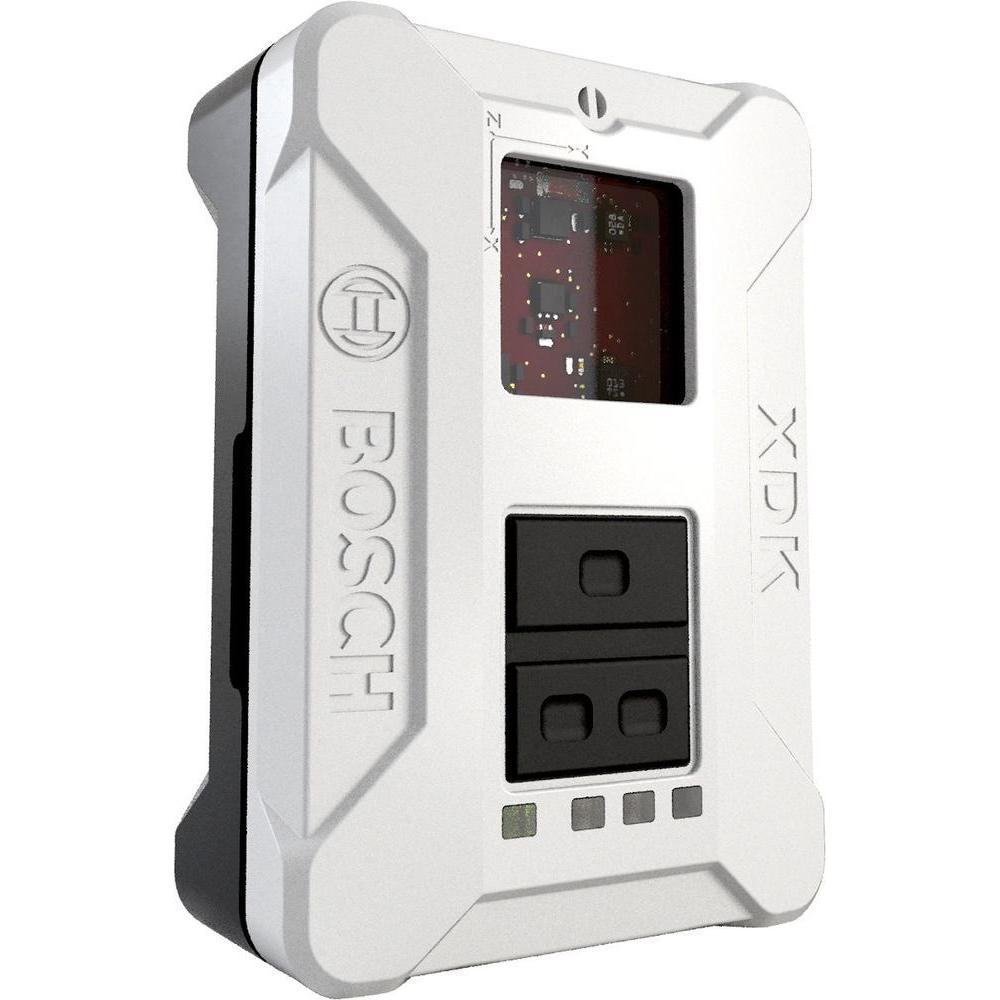
\includegraphics[width=5cm]{images/xdk.jpg}	
	\caption{Bosch \acs*{XDK}}
	\label{fig:XDK}
\end{figure}
Das Bosch \acf{XDK} ist ein kabelloses Sensor-Kit, welches Rapid Prototyping von Produkten im Rahmen des \acf{IOT} ermöglicht. Es ist ausgelegt für die Entwicklung von Prototypen vor der tatsächlichen Serienentwicklung. 
Hierfür wird die eigens dafür entwickelte Entwicklungsumgebung, die sogenannte XDK-Workbench verwendet. Zur Implementierung der eigenen Software kann zwischen den beiden Programmiersprachen C sowie Eclipse Mita verwendet werden, wobei letztere im Kontext des XDK oft auch als XDK Live bezeichnet wird. Im Rahmen der Studienarbeit haben wir uns für die Programmiersprache C entschieden, da hierfür die Dokumentation noch ausführlicher ausfällt.
\subsection{\acs{XDK} Workbench}\label{subsec:XDK Workbench}
\begin{figure}[H]
	\centering
	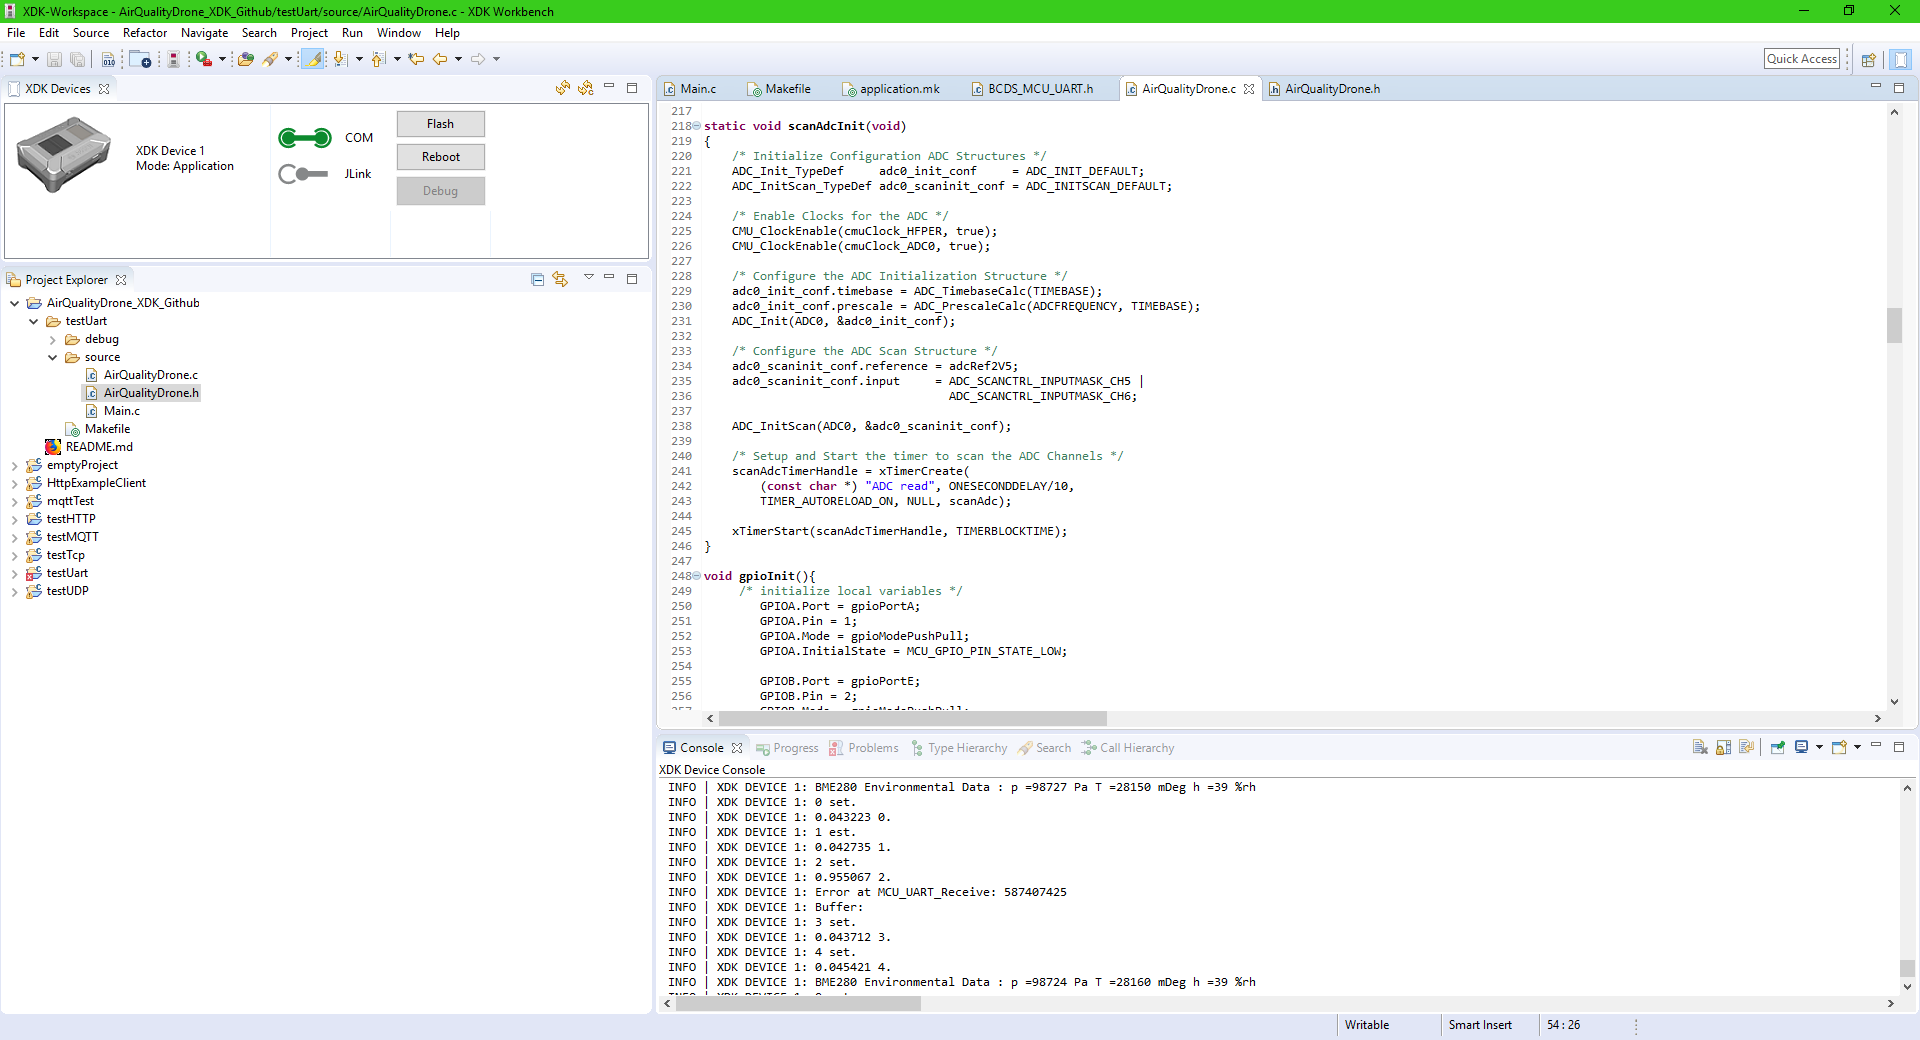
\includegraphics[width=12cm]{images/XDK_Workbench.png}	
	\caption{Bosch \acs*{XDK} Workbench}
	\label{fig:XDK_Workbench}
\end{figure}
Die \acs{XDK} Workbench ist eine auf Eclipse basierende Entwicklungs-Umgebung, um Programmcode für das XDK zu entwickeln, zu debuggen und den Code auf das Gerät zu flashen.
Um ein lauffähiges Programm aus dem Programmcode zu generieren muss das Projekt nach jeder kleinen Änderung zunächst gebuildet werden, bevor man es anschließend über den Flash-Button auf das Gerät laden kann. Um die beim Built erzeugten Binärdateien erfolgreich auf das Gerät zu übertragen, muss sich dieses zunächst im Bootloader-Modus befinden. Diesen kann man herstellen, indem das Gerät ausgeschaltet wird und es anschließend unter Drücken von Button 1 des Gerätes wieder eingeschaltet wird.\newline
Einen wirklichen Debug-Mechanismus bietet die Workbench alleine bis dato nicht. Um dennoch zu debuggen muss ein externes Debug Gerät angeschlossen werden wie beispielsweise die J-Link Debug Probe. \newline
Falls nicht auf dieses externe Debug-Gerät zurückgegriffen werden kann bleibt nichts anderes übrig als über Kommandozeilen-Ausgaben das Programm zu debuggen. Dies ist im Falle des XDK besonders mühsam, da nach jeder kleinen Änderung das Programm wieder gebuildet werden muss, das XDK in den Bootloader-Modus versetzt werden muss und das Programm abschließend geflasht werden muss. Für diesen Prozess können mitunter mehrere Mintuen vergehen, falls beispielsweise noch ein Clean erforderlich ist.
\subsection{Sensoren}\label{subsec:Sensoren}
Das \acs*{XDK} ist mit Sensoren zur Messung folgender Größen ausgestattet:
\begin{itemize} 
	\item Beschleunigung (BMA280)
	\item Gyroskop (BMG160)
	\item Magnetische Feldstärke (BMM150)
	\item Licht (MAX44009)
	\item Sound (AKU340)
	\item Temperatur (BME280)
	\item Relative Luftfeuchtigkeit (BME280)
	\item Luftdruck (BME280)
\end{itemize}
Im Rahmen dieser Arbeit werden die letzten drei genannten Sensoren verwendet, um Informationen über unsere Umwelt zu erlangen.
\subsection{Extension Board}\label{subsec:Extension Board}
\begin{figure}[H]
	\centering
	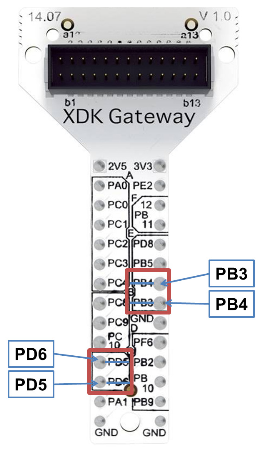
\includegraphics[width=4cm]{images/ExtensionBoard.png}	
	\caption{Bosch \acs*{XDK} Extension Board}
	\label{fig:Extension_Board}
\end{figure}
Zusätzlich zu den eingebauten Sensoren bietet das \acs*{XDK} die Möglichkeit das zugehörige Extensionboard über eine serielle Schnittstelle anszuschließen. Das Extension Board bietet so die Möglichkeit externe Komponenten an den \acs{XDK} anzuschließen, wie beispielsweise weitere Sensoren. Das Board ist bedingt durch die interne \acf{MCU} des \acs{XDK} auf Spannungen zwischen 0V und 2,5V beschränkt, weshalb eingehende Signale mit größeren Spannungen, wie den bei Microcontrollern üblichen 3,3V immer zuerst umgerechnet werden müssen, um den Prozessor nicht zu schädigen. Das Board verfügt über 28 Pins, von denen 23 als \acf{GPIO}-Pins per Software konfiguriert werden können. Neben dieser Standard-Funktionalität der Pins, können einige Pins besondere Funktionalitäten umsetzen, wenn sie entsprechend konfiguriert werden. Das Board verfügt beispielsweise über zwei Pins, die als \acf{ADC} genutzt werden können, mittels deren analoge Spannungspegel gelesen werden. Neben der Möglichkeit analoge Signale zu erkennen, können auch einige Pins serielle Daten auslesen, indem sie beispielsweise als \acf{UART} konfiguriert wurden.

\section{FreeRTOS}\label{sec:FreeRTOS}
Das Betriebssystem des \acs*{XDK} ist FreeRTOS, ein Echtzeitbetriebssystem für eingebettete Systeme. FreeRTOS stellt de facto den Standard für Mikrocontroller und kleine Mikroprozessoren dar nicht zuletzt aufgrund dessen sehr freizügiger Open-Source-Lizenz. Es ist veröffentlicht unter der MIT Lizenz, welche die kostenlose Nutzung der Software selbst zu kommerziellen Zwecken erlaubt. FreeRTOS ist zum größten Teil in der Programmiersprache C entwickelt mit einzelnen Funktionalitäten, die auf Assembler-Ebene umgesetzt sind. Im folgenden betrachten wir die beiden Begriffe Tasks und Timers näher, da diese bei der Entwicklung von Software für den \acs*{XDK} eine große Rolle spielen.
\subsection{Tasks}\label{subsec:Tasks}
Eine auf einem Echtzeitbetriebssystem laufende Applikation kann in mehrere Tasks unterteilt werden. Die Tasks sind unabhängig voneinander und haben jeweils einen eigenen Task-Kontext. Es kann immer nur genau ein Task innerhalb des System aktiv sein, sodass im Falle mehrerer parallel laufender Task ein Scheduler den Tasks zur Laufzeit Rechenleistung zuweist und entscheidet, welcher Task gerade aktiv ist. 
\subsection{Timers}\label{subsec:Timers}
Ein Timer wird verwendet, wenn eine Funktion zu einem festen Zeitpunkt ausgeführt werden soll. Die Funktion, die nach Ablauf des Timers ausgeführt wird, bezeichnet man als Callback-Funktion. Neben Timern, die ein einmaliges Ereignis zu einem festen Zeitpunkt triggern, ist es möglich den Timer zu resetten, sodass die Callback-Funktion periodisch aufgerufen wird.
